\documentclass{article}
% 11-785 Project Proposal Template
% https://www.overleaf.com/latex/templates/11-785-project-proposal-template/gvfmxtrwcttd
\usepackage{11785_project,times}
\usepackage{hyperref}
\usepackage{url}
\usepackage{graphicx}

\graphicspath{ {./img}}

\title{COMP590--171 Project Proposal: Refraction Networking}

\author{Dohhyun Kim, Harin Lim, Jesse Wei, Daniel Xie, Matseoi Zau}

\date{April 4, 2024}

\begin{document}

\maketitle

\section{Refraction networking introduction}

Refraction networking (RN) is a scheme for evading censorship technology, such as website blacklists enforced by governments, with the help of an ISP partner. Specifically, in refraction networking (also called ``decoy routing''), the user requests a blocked site, but the RN protocol actually requests a reachable site with some encrypted header information. The censor accepts the request that seems to be legitimate, but the ISP partner reads the header information and ``refracts'' the request to the blocked site that the user originally requested.

\begin{figure}[h]
    \centering
    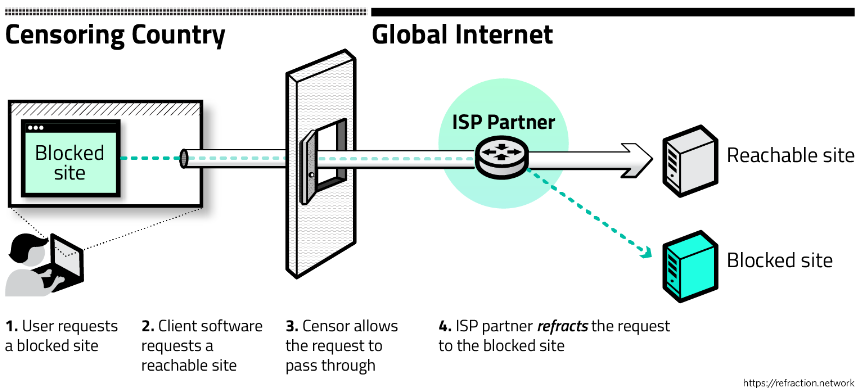
\includegraphics[width=0.8\textwidth]{refraction_networking}
    % TODO: make this not show up as [ref]
    % Note that adding author as "Refraction Network Team" makes the reference [team]
    \caption{Refraction networking \cite{refraction_network}}
\end{figure}

The specific RN protocol we will reimplement for our project is TapDance \cite{tapdance}.

\section{Reimplementation of TapDance}

\section{Member Roles}

\begin{itemize}
\item Dohhyun Kim - 
\item Harin Lim - 
\item Jesse Wei - 
\item Daniel Xie - 
\item Matseoi Zau - 
\end{itemize}

\section{Project Timeline}

\begin{itemize}
\item 2024/04/04 - Submit Proposal 
\item 2024/04/04 - Milestone 1 
\item 2024/04/04 - Milestone 2  
\item 2024/04/04 - Milestone 3  
\item 2024/05/?? - Final Presentation 
\end{itemize}

\newpage
\printbibliography

% \bibliographystyle{11785_project}

\end{document}
